\section{Technical Details of the Optimizer}
\label{sec:tech-details}
The sections above describe my innovations in model construction and simulation, as well as the experimental data brought to bear on optimization. These data are used to parameterize NeuronUnit tests, one per measurement type.
For example, input resistance data for one neuron type in NeuroElectro, or one specific neuron in the Cell Types database, is passed to an \textit{InputResistanceTest} defined in NeuronUnit.
This test ``asks" the model to generate a corresponding simulation, measures the input resistance in this simulation output, and then assesses model/data agreement, resulting in a score.
These mechanics have been described at length previously in \cite{omar2014collaborative}, \cite{gerkin_neuronunit}, and \cite{birgiolas2019towards}.

\subsection{Generating and Using Scores}
\begin{figure}
\begin{center}
    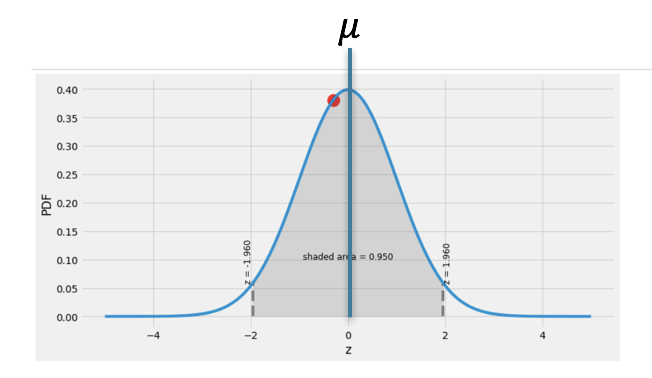
\includegraphics{figures/normal_distribution}
    \caption[Z-scores for NeuronUnit Tests]{\textbf{Z-scores for NeuronUnit Tests}. As discussed in the section \ref{sec:neuronunit}, error functions were evaluated with the assistance of the \emph{NeuronUnit} library.
    This involves obtaining an experimental distribution over electrophysiology feature measurements for a cell type, measuring corresponding model output features, and then locating those features in that experimental distribution. 
    Scores that are closer to the experimental mean are identified as low error.
	The Z-score encodes this information; a Z-score of 0 is the lowest possible error.}
	\label{fig:normal-dist}
\end{center}
\end{figure}
%XXXX Something about Z-score vs RatioScore.

One way to ask whether the simulated feature is a good match to the biological data distribution is to use a Z-score.
The Z-score is defined as:
\begin{equation}
Z-Score = \frac{s - b_{\mu}}{b_{\sigma}}
\end{equation}
where $s$ is the value of the feature in the model simulation, and $b_{\mu}$ and $b_{\sigma}$ are the mean and standard deviation of that feature in the biological data distribution.
The Z-score does not specifically assume that the biological data are normally distributed, although this generates the most natural interpretations.
%(Figure \ref{fig:normal-dist}).
In cases when the biological data from one neuron type comes from a single experiment on a single neuron (as with some data from the Allen Cell Types database or the Blue Brain Project), there is no mean or standard deviation, so I compute a \emph{RatioScore}:
\begin{equation}
Ratio-Score = \frac{s}{b}
\end{equation}%%%Fixed error
where $b$ is the observed biological feature value.
Both types of scores were then normalized to produce an error signal in the range $(0, \inf)$ for use by the optimizer.
For example, suppose a feature(e.g. the rheobase current) had value $\mu \pm \sigma = (100pA \pm 40pA)$ in the biological data, and $110 pA$ in the simulated model output.
Then the following steps were taken to transform it into an error signal:
\begin{enumerate}
 \item A Z-score is computed: $\frac{110 pA - 100 pA}{40 pA} = 0.25$
 \item This is converted to the range (0, 1) using the error function: $abs(erf(Z)) = 0.27$ 
 \item The logarithm is computed: $\log_{10}(0.27) = 0.56$ 
\end{enumerate}
The value 0.56 above represents a larger model/data disagreement than the ``best" possible value of 0 (corresponding to a Z-score of 0), but less disagreement then the ``worst" possible value of $\inf$ (truncated in practice at 100) representing a Z-score of $+\infty$ or $-\infty$. The summed error signal over all $n$ NeuronUnit tests (e.g. rheobase, input resistance, spike rate adaptation, etc.) is:
\begin{equation}
Total  Error = \sum_i^n error_i
\end{equation}
i.e. the sum of all of the errors.  Again, 0 would represent perfect model/data agreement across all tests.

While the optimizer attempts to minimize the total error of the model according to the equation above, evaluation of the quality of the optimized model is evaluated using a hypothesis testing framework.
Specifically, I ask whether there is sufficient evidence that the optimized model is representative of the distribution of feature values observed in the biological data.
The null hypothesis can be states as ``the observed features of the optimized model were drawn from the distribution of features of biological neurons".
In order to generate a test statistic for hypothesis testing, I compute $\chi^{2}$, defined as (in the case of Z-scores):
\begin{equation}
\chi^{2}=\sum\limits_{i=1}^{n}(Z_{i}^{2})
\end{equation}
This equation arises from the fact that a Z-score is simply a standardized normal variable, and a chi-squared distribution with $n$ degrees of freedom is simply the distribution of $n$ independent, squared normal variables.
I compute a p-value by comparing the observed $chi^2$ statistic to the cumulative distribution function of the $chi^2$ distribution with degrees of freedom equal to the number of NeuronUnit tests used (which is equal to the number of Z-scores produced).
If this p-value is small (e.g. $<0.05$), that can serve as evidence to reject the null hypothesis, indicating that the optimized model did not ``fit in" well with the observed biological data.
In contrast, failure to reject the null hypothesis would suggests that the optimized model was somewhat convincing in its mimicry of a biological neuron, for the features in question.

\subsection{Mechanics of Optimization using NeuronUnit}
Here I will describe how I generate these scores concurrently for many parameterizations of the same model and how they guide the optimization path.
I created two different optimization code bases based on the DEAP Python package for genetic optimization \citep{DEAP_JMLR2012}, one that relied on DEAP directly, and one that relied on the BluePyOpt package produced by The Human Brain Project \citep{bluepyopt} (These have since been merged together), in order to achieve optimization using NeuronUnit.
A few key modules are essential to both approaches.
I wrote the file \emph{optimization-management.py} to contain the logic of and methods for managing complex optimization jobs.
It helps the optimizer handle both fixed and varying  model parameters, contains methods for random sampling of model parameter spaces, can plot models output for visualization of this space, and assists in computing the F-I curve.
I also add several methods for inter-converting between representations of the models themselves and the chromosomes that represent only parameter values.

A created a \emph{NUFeature\_standard\_suite} class to convert NeuronUnit features to BluePyOpt objective functions, as outlined in simpler terms in the enumerated list above.
These classes contain a complicated nesting of fault handling statements, as there are many reasons why a candidate model could return unusable simulation output (typically non-biological parameter values), resulting in values like $NaN$ and $\inf$; such values must be recast as poor but finite errors so that the optimizer can see a smooth error surface.
There are two flavors of \emph{NUFeature\_standard\_suite}, one for supra-threshold simulation experiments and another for at threshold or sub-threshold experiments, since each experiment type produces different feature requiring different feature extractors, and producing different sets of edge cases to be handled independently.
For example, there are more ways for a model to fail to elicit multiple action potentials (causing all ISI-based feature extraction functions to return $NaN$ values), than there are to fail to exhibit a hyperpolarizing response to a small outward current injection for the measurement of input resistance.
 
I created a \emph{model-parameters.py} file, a collection of ordered dictionaries, that informed the optimizer which parameters should be modifiable (in the highest-dimensional cases, all of them) and what are reasonable (biologically plausible) search boundaries.
This file also contains example parameter sets representing notable dynamical regimes, such as those shown in \cite{izhikevich2003simple}.
I also made this file and its methods inter-operable with BluePyOpt model parameter management scheme.

\subsubsection{Optimization Parameters}
Optimization requires searching for better and better solution across multiple generations of chromosomes (parameter sets), as noted in section \ref{sec:genetic-algorithms}.
Robust optimization for the models used here required $NGEN\sim150$ generations with a population size (number of parameter sets explored in each generation) of $\mu=35$.
In other words, it took about $150$ generations of mutation, crossover, and selection to achieve convergence, and in each generation about $35$ models had each of their feautures computed and scored.
These parameter values achieved an acceptable balance between exploration of the parameter space and exploitation of favorable regions.
In some cases, values as small as $NGEN=10$ and $\mu=10$ were tolerable, for example when optimizing only low-dimensional cross-sections of parameter space.
In other cases, such as when the number of optimization objectives (i.e. the number of electrophysiological features being tested) was $NOBJ>25$, values as high as $NGEN=300$ and $\mu=100$ were required to obtain adequate results.

\subsubsection{Multiobjective Scoring and Selection}
One potential scientific goal is to maintain a diverse set of solutions (i.e. very different parameter sets that nonetheless each produce simulations that adequately match observed experimental measurements).
The optimization literature has developed many competing approaches for doing this \citep{deb2000fast}, but it usually involves two popular algorithms, named IBEA and NSGA2, which I investigated here.
NSGA2 uses some additional ranking mechanisms, to re-weight the perceived fitness of each chromosome and influence the probability that it survives (or is bred into) the next generation.
For example, it tries to minimize ``crowding distance", penalizing chromosomes that aggregate in clusters, as persistent cluster formation means that the GA becomes preoccupied with more limited regions of the solution space, harming solution diversity.
Another meta-constraint called ``non-dominated sorting" ranks most highly each chromosomes that is not unanimously defeated by any other chromosome on any feature score.
For example, though one parameter set $P$ might produce a model which score poorly on all features except Input Resistance, if no other parameter set has a higher-scoring Input Resistance feature then $P$ is retained. Consistent with personal communication with \cite{van2007neurofitter}, adding in crowding distance and non-dominated sorting typically harms optimizer performance, in the context of neuronal model optimization, though the reason for this is not argued conclusively, I speculate on a likely cause in the discussion of this work.
A simpler ``select best" algorithm (labelled IBEA) dispenses with these tricks, performs no meta-constraint scoring, and simply retains the fittest chromosomes for mutation, crossover, and selection. This simpler selection algorithm was found to work well when optimizing reduced neuronal models.

\subsection{Comparison to Previous Approaches to Optimization}

\subsubsection{Time-dependent Mutation}
Other labs have previously developed schemes to optimize neuron models, e.g. \cite{druckmann2007novel}.
I retained the conceptual insights of these approaches where they were useful for the problems at hand.
For example, I utilized a time-dependent mutation magnitude ($\eta$).
The idea is that big mutations are more helpful in the early stage of optimization, when it is important to explore the vast hyper-volume of parameter sets and get a general picture of the error surface, and that these mutations should be smaller during the later ``refinement" stage of optimization, as the best solutions are approached. Time diminishing $\eta$ did improve genetic algorithm on reduced model optimization problems.

\subsubsection{Variants on Somatic Current Injection}
Nearly all neuron optimization work (including this one) relies on the responses to somatically-injected current as the domain for optimization.
This is largely motivated by the existence of a common and simple experimental analogue using patch clamp (which drives experimental design for both the Allen Cell Types Database and The Blue Brain Project).
But there are three different strategies for choosing the subset of these experiments that are recapitulated in optimization.

% The first strategy was to assume that measurements of an at threshold rheobase spike were sufficient to fit the model to the entire F-I curve, and if all neurons showed an identical regular, non-accommodating spiking pattern, this strategy would might be sufficient to identify a model, with all the right at threshold and above threshold dynamics. To the extent that this assumption is violated, various additional above-threshold current injections will be needed, these are described in strategies two and three. 

% The second strategy involves first identifying the rheobase currents per model and choosing two extra multiples of rheobase current reserved for further model evaluation. This strategy is more direct and slightly more rapid, but it is inefficient in terms of constraining the model, because all of the "action" in the F-I curve occurs above rheobase, but not too far above rheobase (i.e. not at currents that induce depolarization block).

% The third strategy is like the second, but deliberately samples single above threshold locations on the F-I curve (any location that elicits one spike). It is actually the third strategy that was used to produce multi spiking fits, in this work. 

% The fourth strategy involves making an informed guess to make a fixed set of current amplitudes (e.g. ascending 100 pA steps) from the data and probing the model with these, then comparing model and data within this subset. 

%Here I have described four different strategies for constraining models, 
In the optimization framework I tested many different strategies for constraining models with current injections, there were only two important differences between all four strategies: one type of strategy constrains cell behavior at multiple values of current injection, and the other strategy constrains cell behavior at a single current injection value (rheobase or otherwise). Each strategy seeks to resolve a ``bias variance trade-off" differently, and so knowledge of bias variance trade-off is important for understanding the dramatically different quantities of fit found.

When only one current injection value is used seemingly great fits of spike shape, and spike time can be achieved, because the reduced models are more able be over-fitted with respect to a limited range of data. When a model is constrained relative to multiple current injection values, over-fitting of the model is less possible. The optimizer produces a model that is compromised on almost all constraints, with few exceptions. %Because of design choices in multispiking optimization the main constraint that is robust against being compromised is the current versus firing rate relationship. This result is compatible with other findings in the literature probably many optimizer compromises have lead to spike shape being poorly recovered by the optimizer but spike times are perfectly recapitulated \citep{rossant2011fitting}. 

Deliberately over-fitting models was an important optimization strategy in the earlier development of the optimizer, as at the time the highest priority was to verify that the optimizer was functional in a multi-spiking context, however, now with functionality well established producing less good but more generalized fits will become a higher imperative.

% , but the majority of other fitness values will be heavily compromised
%%
% Not inefficient at constraining model, but efficient at 
%%


%This strategy was used not just in optimization, but also in the analysis and re-organization of existing ephys data.
% Action potential waveforms are most regular and consistent in shape when evaluated very near rheobase. Are they? 

%If one follows a multiple current injection optimization strategy, one must also decide how many current amplitudes (above rheobase) must be evaluated in order to adequately constrain model parameters.

% 

%There is an further issue

% the second and third strategy, 

% It attempts to identify the minimum current required to cause some target spike number observed in a dataset. With matching spike counts across simulated and biological data, downstream feature analysis (e.g. spike rate adaptation indices) are likely to be more directly comparable. The consequences of these decisions are explored in the Results section.


%Differences in spike shape and spike timing statistics are thus only modulated by differences in model parameters.

\subsection{Feature Extraction}
Each NeuronUnit test used in the optimizer represents the evaluation of a single feature of simulated output, for example the Input Resistance.
I greatly extended the number of such features/tests covered by NeuronUnit in order to produce a rich, multi-objective optimizer that could capture important spiking dynamics and to obtain insights into what would be the most compact subset for subsequent use in unique identification of models.

\subsubsection{Elephant Features Test Suite}
\label{sec:elephant}
Elephant \citep{elephant18} provides feature extraction capabilities for membrane potential time series expressed using the Neo library in Python \citep{davison_neo}.
Eight NeuronUnit tests (five used here) are derived from Elephant feature extraction, particularly those associated with passive membrane properties assessed with subthreshold stimuli, or action potential waveform properties assessed at rheobase.
Fundamental quantities such as capacitance or input resistance are among these, though they are not ``emergent properties" of the model since they are roughly predictable from the parameters of the model equations.

\subsubsection{Electrophysiology Feature Extraction Library (EFEL)}
\label{sec:efel}
%Most suprathreshold dynamics were summarized by descriptive statistics of patterns of action potentials. For example, the coefficient of variation of the inter-spike intervals in a spike train can serve as a measure of "burstiness". -- No EFEL has many spike shape qualities. as the noted well as spike train statistics. I'd say the ratio of spike train statistics to spike shape measurements is about 1:1.
The Blue Brain Project developed the Electrophysiology Feature Extraction Library (EFEL) to compute many such statistics from spike trains, and I used these to generate tests of suprathreshold dynamics for optimization \citep{EFEL}.

\subsubsection{Allen Institute Software Development Kit (Allen SDK)}
\label{sec:allensdk}
The Allen Institute offers yet another set of tools for feature extraction, applying to both sub- and suprathreshold features of neuron responses to current injection.
The reason to use Allen features in addition to the above is that some of these features are predicated on particular current stimuli (e.g. a stimulus that is exactly 20 pA stronger than the rheobase current).
% I don't think the following is needed, and it may be misconceived.

% Here is why: In the Allen sweep data sets, the current that produced the voltage is known and stored (think of it as a current V_M pair), it is not thrown out. 

% In any case, if you have Allen data and Allen features, or Allen data and EFEL features. Comparing the original voltage trace is still possible, comparing to the original current is still possible. The main thing that _is_ lost is the opportunity to align findings with official Allen features, but that's it.
Such stimuli either were or were not delivered to the various experimentally recorded neurons, and for the purposes of this thesis there is no going back and delivering additional ones.
Consequently, for model testing and optimization it makes sense to use features--and the stimuli that generated them--that can be directly compared to the recorded neurons.
For the biological neurons in the Allen Cell Types database, these features are available in the Allen SDK.
